\section{System Model - Method 2}
\label{sec:system_model}

This chapter shows an alternative approach to the system model using beta distributed noise on the lateral velocity to better mimic driver response to stay in the centre of the road. The model describes the motion of a vehicle constrained to a closed loop 2D track, expressed entirely in path-frame coordinates $(s,l)$, where $s$ is the position along the track and $l$ is the lateral position on the track, normal to the direction of movement. 

% ---------------------------------------------------------------------
\subsection{State Vector and Process Equations}
\label{subsec:state_model}

The path-frame coordinates ($s$,$l$) express the vehicle state in a path-aligned reference frame attached to the track center line. This removes the need to embed the curvature of the track inside the dynamics themselves and simplifies the model ensuring the vehicle follows the track.  The state vector is:
\begin{equation}
    \mathbf{x}_k \;=\; \begin{bmatrix} s_k \\ v_k \\ l_k \\ v_{l,k} \end{bmatrix},
    \label{eq:state_vector}
\end{equation}
where $s_k$ is the arc-length position along the center-line of the track (in meters), $v_k$ is the longitudinal speed along the track, $l_k$ is the lateral position normal to the center-line (with $+l$ to the left of the direction of motion) and $v_{l,k}$ is the lateral speed. The lateral position must be within +/- half the track: $|l_k|\leq l_{\max}$.

The discrete-time process model is:
\begin{align}
    s_{k+1}    &= \bigl( s_k + h\,v_k \bigr) \bmod L_{\text{total}}, \label{eq:s_update} \\
    v_{k+1}    &= v_k + w_{v,k}, \qquad w_{v,k} \sim \mathcal{N}\!\left(0,\sigma_v^{2}\right), \label{eq:v_update} \\
    l_{k+1}    &= l_k + h\,v_{l,k}, \label{eq:l_update} \\
    v_{l,k+1}  &= v_{l,k} + w_{l,k}(l_k), \label{eq:vl_update}
\end{align}
with $L_{\text{total}}$ the total length of the closed loop. The arc-length update in~\eqref{eq:s_update} wraps modulo $L_{\text{total}}$ so that the vehicle may complete an unlimited number of laps, producing the characteristic sawtooth signal in $s_k$. The longitudinal speed noise term is a zero-mean Gaussian. The nominal cruise speed is set entirely by the initial condition $v_0$, and although $\mathbb{E}[v_k]=v_0$, the variance grows linearly in $k$ so the speed will wander over long horizons. The lateral position in~\eqref{eq:l_update} is the integral of the lateral speed, and the noise term affecting lateral speed follows a state-dependent Beta-based noise $w_{l,k}(l_k)$.

% ---------------------------------------------------------------------
\subsection{Process Noise Distributions}
\label{subsec:noise}

Two scalar parameters control the magnitude of the process noise: the longitudinal Gaussian standard deviation $\sigma_v$ in equation~\eqref{eq:v_update}, and the lateral Beta scale factor $c$ (\texttt{beta\_scale})

\paragraph{Longitudinal noise scale $\sigma_v$.}
The longitudinal driving noise $w_v$ is a standard zero-mean Gaussian and can be described by a single standard deviation $\sigma_v = 0.05m/s$. This equates to +/- $0.05m/s$ or $0.014km/h$ of noise being added to the system every time step $h$. This equates to $+/- 1.4km/h/s$ which is a reasonable value for a human driver trying to maintain a constant speed. 

\paragraph{Lateral noise scale $c$.}
The lateral noise is constructed from a Beta-distributed random variable and is used to bias the vehicle back towards the centre of the track. Given $E[w_t]$ = $a/(a+b)$ for the beta distribution is 0.5, we subtract this from the noise term to ensure that the expected value of $w_t$ for any $l$ goes to 0 i.e. zero-mean, which re-centres the distribution around zero so only the shape depends on $l$:
\begin{equation}
    X \sim \mathrm{Beta}\bigl(a(l),\,b(l)\bigr), \qquad
    w_l \;=\; c \left( X - \frac{a(l)}{a(l)+b(l)} \right),
    \label{eq:beta_noise}
\end{equation}
where $c$ is a fixed scale factor that scales the [0 1] distribution down to reasonable levels, more reprenatative of real world. A value of \texttt{beta\_scale}~$=0.01$~m/s was chosen. This is almost one magnitude smaller than the longitudinal noise term and is more realistic of real-world driving.

\paragraph{Skew and concentration.}
The two Beta shape parameters $a$ and $b$ control two largely independent aspects of the PDF. The ratio of $a$ to $b$ controls the \emph{skew}: $a>b$ moves the probability mass toward the right, producing a distribution whose mode lies above the mean and whose tail extends in the negative direction once the noise has been recentred. $a<b$ does the reverse. When $a=b$ the PDF is symmetric about $0.5$ or $0$ when recentred. The sum $a+b$ controls the \emph{concentration}: a larger sum produces a narrower, peakier PDF, while a smaller sum spreads the mass more uniformly.

\paragraph{Linear interpolation method.}
Rather than prescribing closed-form expressions for $a(l)$ and $b(l)$, the shape parameters are specified directly at three anchor-positions chosen to span the lateral range,
\begin{equation}
    l \in \{\, -l_{\max},\; 0,\; +l_{\max} \,\},
\end{equation}
and any intermediate $a(l)$, $b(l)$ is obtained by linear interpolation between the anchors. Where track width $w=4$~m and therefore $l_{\max}=w/2=2$~m. Linear interpolation was selected for its simplicity. It produces continuous shape variation across the track without introducing additional tuning parameters and makes the effect of each anchor easy to tune in isolation.

The three sets of $(a,b)$ values used in the simulation are listed in Table~\ref{tab:anchors}.

\begin{table}[h]
    \centering
    \begin{tabular}{c|cc}
        $l$         & $a(l)$ & $b(l)$ \\ \hline
        $-l_{\max}$ & 5      & 1      \\
        $0$         & 50     & 50     \\
        $+l_{\max}$ & 1      & 5
    \end{tabular}
    \caption{Beta shape parameters at the three anchor positions.}
    \label{tab:anchors}
\end{table}

\begin{figure}[H]
    \centering
    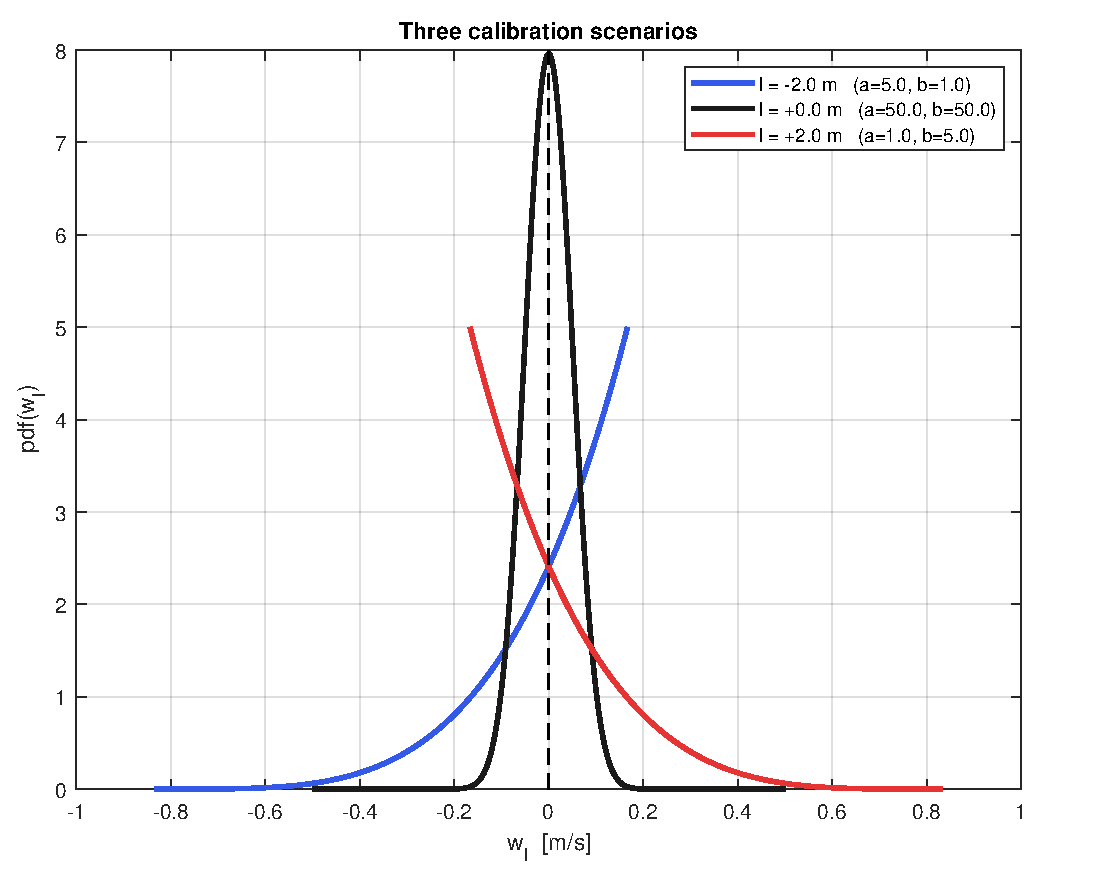
\includegraphics[width=0.8\textwidth]{figures/beta_cal.pdf}
    \caption{Beta probability density functions at the three lateral
             anchor positions.}
    \label{fig:beta_scenarios}
\end{figure}

At the centre of the track ($l=0$) the distribution is symmetric and very concentrated ($a+b=100$), so the lateral kick is small in magnitude and unbiased. At each of the walls the distribution becomes strongly skewed in the direction that pushes the vehicle back towards the centreline. This produces an effective restoring tendency while still ensuring the noise still has zero-mean, which keeps the dynamic model simple. 

% ---------------------------------------------------------------------
\subsection{Measurement Equation}
\label{subsec:measurement}

The vehicle is tracked using $M$ fixed beacons placed at known world-frame coordinates $\mathbf{b}_i = [\,b_{i,x},\, b_{i,y}\,]^{\top}$, $i=1,\ldots,M$. At each discrete time step $k$, every beacon reports a noisy range to the vehicle:
\begin{equation}
    y_{i,k} \;=\; \sqrt{\bigl(x_k - b_{i,x}\bigr)^{2} + \bigl(y_k - b_{i,y}\bigr)^{2}} \;+\; n_{i,k}, \qquad n_{i,k} \sim \mathcal{N}\!\left(0,\sigma_y^{2}\right),
    \label{eq:meas_scalar}
\end{equation}
where $(x_k, y_k)$ is the world-frame position of the vehicle, obtained from the path coordinates $(s_k, l_k)$ via the mapping, and $n_{i,k}$ is independent zero-mean Gaussian noise with standard deviation $\sigma_y$. Stacking the $M$ beacon ranges into a vector $\mathbf{y}_k \in \mathbb{R}^{M}$ gives the measurement model in compact form:
\begin{equation}
    \mathbf{y}_k \;=\; \mathbf{h}(\mathbf{x}_k) + \mathbf{n}_k, \qquad \mathbf{n}_k \sim \mathcal{N}\!\left(\mathbf{0},\,\sigma_y^{2}\,\mathbf{I}_{M}\right).
    \label{eq:meas_vector}
\end{equation}

The mapping $\mathbf{h}(\cdot)$ is non-linear because the Euclidean range $\sqrt{(\cdot)^{2} + (\cdot)^{2}}$ is itself a non-linear operation.

% ---------------------------------------------------------------------
\subsection{Track Geometry and Path-to-World Mapping}
\label{subsec:track}

The track is a closed planar loop formed by a large semicircle of radius $R_1=50$~m, a small semicircle of radius $R_2=20$~m, and the two external-tangent straight segments that join them. The two circle centres lie on the $x$-axis and are separated by a distance $D=100$~m. With $R_1\neq R_2$ the connecting straights are not horizontal but inclined at an angle
\begin{equation}
    \alpha \;=\; \arcsin\!\left(\frac{R_1 - R_2}{D}\right)
    \label{eq:alpha}
\end{equation}
This means that the two circular arcs do not meet the straight sections at the top-most and bottom-most points i.e. when the arc lengths are $\pi$ radians. The large arc joins slightly inside giving length $(\pi+2\alpha)$ and the small arc joins slightly outside giving length $(\pi-2\alpha)$. Each connecting straight has length
\begin{equation}
    L_{\text{str}} \;=\; \sqrt{D^{2} - (R_1 - R_2)^{2}},
\end{equation}
and the total closed-loop length is
\begin{equation}
    L_{\text{total}} \;=\; 2 L_{\text{str}} \;+\; (\pi + 2\alpha)\,R_1 \;+\; (\pi - 2\alpha)\,R_2.
\end{equation}

\paragraph{The \texttt{sl\_to\_xy} mapping.}
Because the dynamics are in $(s,l)$ coordinates, a mapping is required to get world-frame coordinates $(x,y)$. The arc-length parameter $s$ is partitioned into four contiguous sections in order of increasing $s$:
\begin{enumerate}
    \item the bottom straight, $s\in[0,\;L_{\text{str}}]$;
    \item the small (right-hand) arc, $s\in[L_{\text{str}},\;L_{\text{str}} + L_{\text{arc},2}]$;
    \item the top straight, $s\in[L_{\text{str}} + L_{\text{arc},2},\;2L_{\text{str}} + L_{\text{arc},2}]$;
    \item the large (left-hand) arc, $s\in[2L_{\text{str}} + L_{\text{arc},2},\;L_{\text{total}}]$,
\end{enumerate}
where $L_{\text{arc},2}=(\pi-2\alpha)R_2$ is the small-arc length. 
For a query value of $s$, the function first reduces it modulo $L_{\text{total}}$ to ensure it lies inside one period of the loop, then finds the section in which it falls to evaluate the centre-line position $\mathbf{p}(s)$ and the tangent heading $\psi(s)$. On the straight sections $\mathbf{p}(s)$ is a linear interpolation between the two tangent points of that segment and $\psi(s)$ is the constant heading of the segment; on the arcs $\mathbf{p}(s)$ is a circular position calculated by an angle that advances as $s$ increases, and $\psi(s)$ is that angle plus $\pi/2$, giving the local tangent direction.

The world position at lateral offset $l$ is then obtained by displacing $\mathbf{p}(s)$ along the unit normal pointing to the left of $\psi$ (the positive $l$ direction):
\begin{equation}
    \begin{bmatrix} x \\ y \end{bmatrix}
    \;=\;
    \begin{bmatrix} p_x(s) \\ p_y(s) \end{bmatrix}
    \;+\; l
    \begin{bmatrix} -\sin\psi(s) \\ +\cos\psi(s) \end{bmatrix}.
    \label{eq:sl_to_xy}
\end{equation}

\paragraph{Track-width constraint.}
The lateral dynamic equation places no limit on $l_k$ which over time has a non-zero probability of going outside the track. To prevent this, after each step the value of $l_{k+1}$ is tested against the wall constraint $l_{max} =2m$. Whenever a the wall it hit, the lateral speed is reflected by changing sign and reducing magnitude: $-0.2vl$. This acts to absorb most of the lateral kinetic energy on contact preventing the vehicle from sticking to the wall or jumping off wildly across the track.

% ---------------------------------------------------------------------
\subsection{Initial State}
\label{subsec:initial}

The simulation is initialised with
\begin{equation}
    \mathbf{x}_0 \;=\; \begin{bmatrix} s_0 \\ v_0 \\ l_0 \\ v_{l,0} \end{bmatrix}
    \;=\; \begin{bmatrix} 0 \\ 10~\text{m/s} \\ 0 \\ 0 \end{bmatrix}.
    \label{eq:x0}
\end{equation}
The vehicle starts at the origin of the path coordinate (the start of the bottom straight), perfectly aligned with the centre-line ($l_0 = v_{l,0} = 0$), and travelling at $v_0 = 10$~m/s, or roughly $36$~km/h. Because the noise in the longitudinal dynamic equation is zero-mean, we know that the initial velocity becomes the expected value  $\mathbb{E}[v_k] = v_0$ for all $k$. The initial condition therefore sets the nominal cruise speed for the entire simulation with no separate setpoint or control input required.

To forbid both reverse motion and unrealistically high speeds the longitudinal speed must be limited as follows:
\begin{equation}
    0 < v_k \;\leq\; 25~\text{m/s}
\end{equation}
However, with the chosen $\sigma_v = 0.02$~m/s and the small simulation horizons the trajectory remains many standard deviations away from either bound throughout. The clamp could be re-introduced as a hard constraint if longer horizons or larger values of $\sigma_v$ are used.

% ---------------------------------------------------------------------
\subsection{LLM Usage}
\label{subsec:llm usage}

LLMs were used to draft the matlab scripts and create the animation plots. During the state model derivation LLMs were used to query and appraise different approaches. LLMs were also used to draft the Latex equations for the final report.